% This file was created with tikzplotlib v0.10.1.
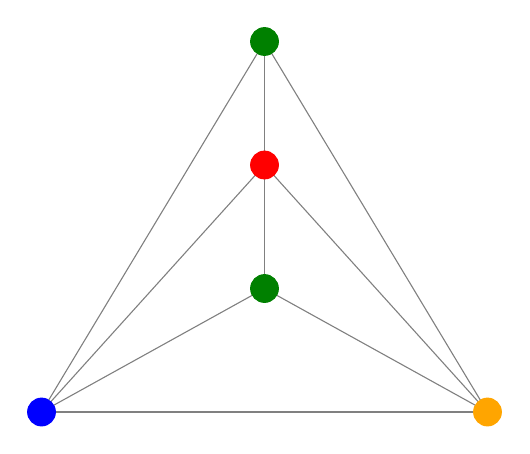
\begin{tikzpicture}

\definecolor{darkgray176}{RGB}{176,176,176}
\definecolor{gray}{RGB}{128,128,128}

\begin{axis}[
hide x axis,
hide y axis,
mark size=5pt,
scaled x ticks=manual:{}{\pgfmathparse{#1}},
scaled y ticks=manual:{}{\pgfmathparse{#1}},
tick align=outside,
x grid style={darkgray176},
xmajorticks=false,
xmin=-1.21, xmax=1.21,
xtick style={color=black},
xticklabels={},
y grid style={darkgray176},
ymajorticks=false,
ymin=-0.505, ymax=0.705,
ytick style={color=black},
yticklabels={}
]
\path [draw=gray]
(axis cs:-1,-0.4)
--(axis cs:1,-0.4);

\path [draw=gray]
(axis cs:-1,-0.4)
--(axis cs:0,-0.0666666666666667);

\path [draw=gray]
(axis cs:-1,-0.4)
--(axis cs:0,0.266666666666667);

\path [draw=gray]
(axis cs:-1,-0.4)
--(axis cs:0,0.6);

\path [draw=gray]
(axis cs:1,-0.4)
--(axis cs:0,-0.0666666666666667);

\path [draw=gray]
(axis cs:1,-0.4)
--(axis cs:0,0.266666666666667);

\path [draw=gray]
(axis cs:1,-0.4)
--(axis cs:0,0.6);

\path [draw=gray]
(axis cs:0,-0.0666666666666667)
--(axis cs:0,0.266666666666667);

\path [draw=gray]
(axis cs:0,0.266666666666667)
--(axis cs:0,0.6);

\addplot [
  mark=*,
  only marks,
  scatter,
  scatter/@post marker code/.code={%
  \endscope
},
  scatter/@pre marker code/.code={%
  \expanded{%
  \noexpand\definecolor{thispointdrawcolor}{RGB}{\drawcolor}%
  \noexpand\definecolor{thispointfillcolor}{RGB}{\fillcolor}%
  }%
  \scope[draw=thispointdrawcolor, fill=thispointfillcolor]%
},
  visualization depends on={value \thisrow{draw} \as \drawcolor},
  visualization depends on={value \thisrow{fill} \as \fillcolor}
]
table{%
x  y  draw  fill
-1 -0.4 0,0,255 0,0,255
1 -0.4 255,165,0 255,165,0
0 -0.0666666666666667 0,128,0 0,128,0
0 0.266666666666667 255,0,0 255,0,0
0 0.6 0,128,0 0,128,0
};
\draw (axis cs:-1,-0.4) node[
  scale=0.6,
  text=white,
  rotate=0.0
]{1};
\draw (axis cs:1,-0.4) node[
  scale=0.6,
  text=white,
  rotate=0.0
]{2};
\draw (axis cs:0,-0.0666666666666667) node[
  scale=0.6,
  text=white,
  rotate=0.0
]{3};
\draw (axis cs:0,0.266666666666667) node[
  scale=0.6,
  text=white,
  rotate=0.0
]{4};
\draw (axis cs:0,0.6) node[
  scale=0.6,
  text=white,
  rotate=0.0
]{3};
\end{axis}

\end{tikzpicture}
